% ============================================================================
% SECTION 0: INTRODUCTION & MOTIVATION
% ============================================================================

\section{Introduction \& Motivation}

% ----------------------------------------------------------------------------
% Slide 0.1: The Problem
% ----------------------------------------------------------------------------
\begin{frame}{The Problem}
    \textbf{Deploying quantized neural networks on microcontrollers is challenging.}
    
    \vspace{1em}
    
    \textbf{Existing tools are inflexible and difficult to extend:}
    
    \begin{itemize}[<+->]
        \item \textbf{TFLite Micro:} Large binary size for microcontrollers usecases, not designed to be extended. As a result,
        extremely difficult to add new quantization techniques.
        
        \item \textbf{Glow:} Complex setup, designed for research not real-world embedded use, hard to add new features.
    \end{itemize}
\end{frame}

% ----------------------------------------------------------------------------
% Slide 0.2: Comparison with Existing Tools
% ----------------------------------------------------------------------------
\begin{frame}{Comparison with Existing Tools}
    \small
    \centering
    \begin{tabular}{l|ccc}
        \toprule
        \textbf{Feature} & \textbf{Tiny-NN-in-C} & \textbf{TFLite Micro} & \textbf{Glow} \\
        \midrule
        \uncover<2->{Framework} & \uncover<2->{PyTorch} & \uncover<2->{TensorFlow} & \uncover<2->{ONNX/PyTorch*} \\
        \uncover<3->{Output} & \uncover<3->{Standalone C} & \uncover<3->{.tflite + Interp.} & \uncover<3->{Compiled binary} \\
        \uncover<4->{Code Readability} & \uncover<5->{\color{deepgreen}\ding{51}} & \uncover<5->{\color{deepred}\ding{55} Binary} & \uncover<5->{\color{deepred}\ding{55} Opt. IR} \\
        \uncover<5->{Setup Complexity} & \uncover<6->{Simple (pip)} & \uncover<6->{Medium} & \uncover<6->{Complex} \\
        \uncover<6->{Binary Size} & \uncover<7->{$\sim$150KB} & \uncover<7->{$\sim$390KB+} & \uncover<7->{Varies} \\
        \uncover<7->{Quantization} & \uncover<8->{int8/16, mixed} & \uncover<8->{int8} & \uncover<8->{int8} \\
        \uncover<8->{Custom Rules} & \uncover<10->{\color{deepgreen}\ding{51} Regex} & \uncover<10->{\color{deepred}\ding{55} Per-layer} & \uncover<10->{\color{deepred}\ding{55} Manual} \\
        \uncover<9->{Extensibility} & \uncover<12->{\color{deepgreen}\ding{51} Easy} & \uncover<12->{\color{deepred}\ding{55} C++} & \uncover<12->{\color{deepred}\ding{55} LLVM} \\
        \uncover<10->{Transparency} & \uncover<14->{\color{deepgreen}\ding{51} See code} & \uncover<14->{\color{deepred}\ding{55} Black box} & \uncover<14->{\color{deepred}\ding{55} Black box} \\
        \bottomrule
    \end{tabular}
    
    \vspace{0.5em}
    \uncover<12->{\footnotesize *Glow development has slowed; PyTorch support via ONNX conversion}
\end{frame}

% ----------------------------------------------------------------------------
% Slide 0.3: Architecture Comparison - TFLite Micro
% ----------------------------------------------------------------------------
\begin{frame}{Architecture Comparison}
    \textbf{TFLite Micro:}
    \begin{center}
    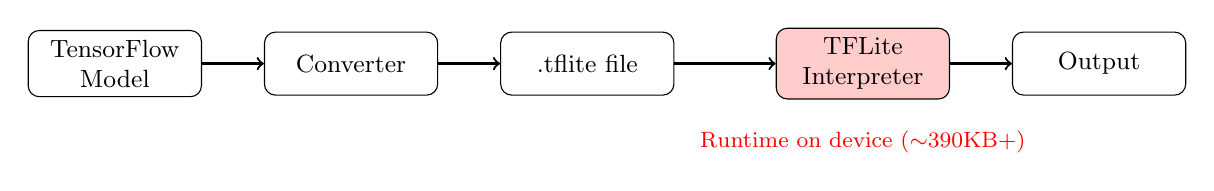
\begin{tikzpicture}[
        box/.style={draw, rounded corners, minimum width=2.2cm, minimum height=0.8cm, align=center, font=\small},
        arrow/.style={->, thick}
    ]
        \onslide<1->{
            \node[box] (tf) at (0,0) {TensorFlow\\Model};
        }
        \onslide<2->{
            \node[box] (conv) at (3,0) {Converter};
            \draw[arrow] (tf) -- (conv);
        }
        \onslide<3->{
            \node[box] (tflite) at (6,0) {.tflite file};
            \draw[arrow] (conv) -- (tflite);
        }
        \onslide<4->{
            \node[box, fill=red!20] (interp) at (9.5,0) {TFLite\\Interpreter};
            \draw[arrow] (tflite) -- (interp);
        }
        \onslide<5->{
            \node[box] (out) at (12.5,0) {Output};
            \draw[arrow] (interp) -- (out);
        }
        \onslide<6->{
            \node[font=\footnotesize, text=red] at (9.5,-1) {Runtime on device ($\sim$390KB+)};
        }
    \end{tikzpicture}
    \end{center}
    
    \vspace{1em}
    
    \onslide<7->{
    \textbf{Glow:}
    \begin{center}
    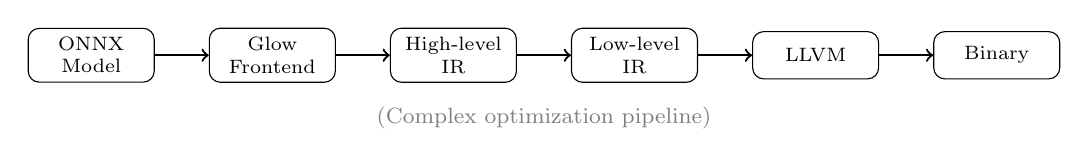
\begin{tikzpicture}[
        box/.style={draw, rounded corners, minimum width=1.6cm, minimum height=0.6cm, align=center, font=\scriptsize},
        arrow/.style={->, thick}
    ]
        \node[box] (onnx) at (0,0) {ONNX\\Model};
        \node[box] (front) at (2.3,0) {Glow\\Frontend};
        \node[box] (hir) at (4.6,0) {High-level\\IR};
        \node[box] (lir) at (6.9,0) {Low-level\\IR};
        \node[box] (llvm) at (9.2,0) {LLVM};
        \node[box] (bin) at (11.5,0) {Binary};
        
        \draw[arrow] (onnx) -- (front);
        \draw[arrow] (front) -- (hir);
        \draw[arrow] (hir) -- (lir);
        \draw[arrow] (lir) -- (llvm);
        \draw[arrow] (llvm) -- (bin);
        
        \node[font=\footnotesize, text=gray] at (5.75,-0.8) {(Complex optimization pipeline)};
    \end{tikzpicture}
    \end{center}
    }
\end{frame}

% ----------------------------------------------------------------------------
% Slide 0.4: Architecture Comparison - Tiny-NN-in-C
% ----------------------------------------------------------------------------
\begin{frame}{Our Approach: Tiny-NN-in-C}
    \begin{center}
    \begin{tikzpicture}[
        box/.style={draw, rounded corners, minimum width=2cm, minimum height=0.8cm, align=center, font=\small},
        optbox/.style={draw, rounded corners, dashed, minimum width=2cm, minimum height=0.8cm, align=center, font=\small, fill=green!10},
        arrow/.style={->, thick},
        optarrow/.style={->, thick, dashed}
    ]
        \onslide<1->{
            \node[box] (pytorch) at (0,0) {PyTorch\\Model};
        }
        \onslide<2->{
            \node[box] (fx) at (3,0) {torch.fx\\Tracer};
            \draw[arrow] (pytorch) -- (fx);
        }
        \onslide<3->{
            \node[box, fill=blue!10] (ir) at (6,0) {IR Graph};
            \draw[arrow] (fx) -- (ir);
        }
        \onslide<4->{
            \node[optbox] (quant) at (6,-1.5) {Quantization};
            \draw[optarrow] (ir) -- (quant);
            \node[font=\scriptsize, text=deepgreen] at (8,-1.5) {Rule-based};
        }
        \onslide<5->{
            \node[optbox] (passes) at (6,-3) {Passes};
            \draw[optarrow] (quant) -- (passes);
            \node[font=\scriptsize, text=deepgreen] at (8,-3) {User-defined};
        }
        \onslide<6->{
            \node[box, fill=orange!20] (ccode) at (10,0) {C Code};
            \draw[arrow] (ir) -- (ccode);
            \node[font=\scriptsize, text=deepgreen] at (10,-0.7) {Readable \& Simple};
        }
    \end{tikzpicture}
    \end{center}
    
    \vspace{1em}
    
    \onslide<7->{
        \begin{block}{Key Insight}
            We achieve \textbf{transparency} and \textbf{simplicity} with minimal performance penalty.
        \end{block}
    }
\end{frame}

